\documentclass[twoside]{book}

% Packages required by doxygen
\usepackage{calc}
\usepackage{doxygen}
\usepackage{graphicx}
\usepackage[utf8]{inputenc}
\usepackage{makeidx}
\usepackage{multicol}
\usepackage{multirow}
\usepackage{textcomp}
\usepackage[table]{xcolor}

% Font selection
\usepackage[T1]{fontenc}
\usepackage{mathptmx}
\usepackage[scaled=.90]{helvet}
\usepackage{courier}
\usepackage{amssymb}
\usepackage{sectsty}
\renewcommand{\familydefault}{\sfdefault}
\allsectionsfont{%
  \fontseries{bc}\selectfont%
  \color{darkgray}%
}
\renewcommand{\DoxyLabelFont}{%
  \fontseries{bc}\selectfont%
  \color{darkgray}%
}

% Page & text layout
\usepackage{geometry}
\geometry{%
  a4paper,%
  top=2.5cm,%
  bottom=2.5cm,%
  left=2.5cm,%
  right=2.5cm%
}
\tolerance=750
\hfuzz=15pt
\hbadness=750
\setlength{\emergencystretch}{15pt}
\setlength{\parindent}{0cm}
\setlength{\parskip}{0.2cm}
\makeatletter
\renewcommand{\paragraph}{%
  \@startsection{paragraph}{4}{0ex}{-1.0ex}{1.0ex}{%
    \normalfont\normalsize\bfseries\SS@parafont%
  }%
}
\renewcommand{\subparagraph}{%
  \@startsection{subparagraph}{5}{0ex}{-1.0ex}{1.0ex}{%
    \normalfont\normalsize\bfseries\SS@subparafont%
  }%
}
\makeatother

% Headers & footers
\usepackage{fancyhdr}
\pagestyle{fancyplain}
\fancyhead[LE]{\fancyplain{}{\bfseries\thepage}}
\fancyhead[CE]{\fancyplain{}{}}
\fancyhead[RE]{\fancyplain{}{\bfseries\leftmark}}
\fancyhead[LO]{\fancyplain{}{\bfseries\rightmark}}
\fancyhead[CO]{\fancyplain{}{}}
\fancyhead[RO]{\fancyplain{}{\bfseries\thepage}}
\fancyfoot[LE]{\fancyplain{}{}}
\fancyfoot[CE]{\fancyplain{}{}}
\fancyfoot[RE]{\fancyplain{}{\bfseries\scriptsize Generated on Fri Jun 24 2016 21\-:26\-:59 for My Project by Doxygen }}
\fancyfoot[LO]{\fancyplain{}{\bfseries\scriptsize Generated on Fri Jun 24 2016 21\-:26\-:59 for My Project by Doxygen }}
\fancyfoot[CO]{\fancyplain{}{}}
\fancyfoot[RO]{\fancyplain{}{}}
\renewcommand{\footrulewidth}{0.4pt}
\renewcommand{\chaptermark}[1]{%
  \markboth{#1}{}%
}
\renewcommand{\sectionmark}[1]{%
  \markright{\thesection\ #1}%
}

% Indices & bibliography
\usepackage{natbib}
\usepackage[titles]{tocloft}
\setcounter{tocdepth}{3}
\setcounter{secnumdepth}{5}
\makeindex

% Hyperlinks (required, but should be loaded last)
\usepackage{ifpdf}
\ifpdf
  \usepackage[pdftex,pagebackref=true]{hyperref}
\else
  \usepackage[ps2pdf,pagebackref=true]{hyperref}
\fi
\hypersetup{%
  colorlinks=true,%
  linkcolor=blue,%
  citecolor=blue,%
  unicode%
}

% Custom commands
\newcommand{\clearemptydoublepage}{%
  \newpage{\pagestyle{empty}\cleardoublepage}%
}


%===== C O N T E N T S =====

\begin{document}

% Titlepage & ToC
\hypersetup{pageanchor=false}
\pagenumbering{roman}
\begin{titlepage}
\vspace*{7cm}
\begin{center}%
{\Large My Project }\\
\vspace*{1cm}
{\large Generated by Doxygen 1.8.5}\\
\vspace*{0.5cm}
{\small Fri Jun 24 2016 21:26:59}\\
\end{center}
\end{titlepage}
\clearemptydoublepage
\tableofcontents
\clearemptydoublepage
\pagenumbering{arabic}
\hypersetup{pageanchor=true}

%--- Begin generated contents ---
\chapter{Hierarchical Index}
\section{Class Hierarchy}
This inheritance list is sorted roughly, but not completely, alphabetically\-:\begin{DoxyCompactList}
\item Q\-Object\begin{DoxyCompactList}
\item \contentsline{section}{Game\-Item}{\pageref{classGameItem}}{}
\begin{DoxyCompactList}
\item \contentsline{section}{Bird}{\pageref{classBird}}{}
\item \contentsline{section}{Land}{\pageref{classLand}}{}
\item \contentsline{section}{Y\-\_\-wood}{\pageref{classY__wood}}{}
\end{DoxyCompactList}
\end{DoxyCompactList}
\item \contentsline{section}{qt\-\_\-meta\-\_\-stringdata\-\_\-\-Game\-Item\-\_\-t}{\pageref{structqt__meta__stringdata__GameItem__t}}{}
\item \contentsline{section}{qt\-\_\-meta\-\_\-stringdata\-\_\-\-Widget\-\_\-t}{\pageref{structqt__meta__stringdata__Widget__t}}{}
\item Q\-Widget\begin{DoxyCompactList}
\item \contentsline{section}{Widget}{\pageref{classWidget}}{}
\end{DoxyCompactList}
\item \contentsline{section}{Ui\-\_\-\-Widget}{\pageref{classUi__Widget}}{}
\begin{DoxyCompactList}
\item \contentsline{section}{Ui\-:\-:Widget}{\pageref{classUi_1_1Widget}}{}
\end{DoxyCompactList}
\end{DoxyCompactList}

\chapter{Class Index}
\section{Class List}
Here are the classes, structs, unions and interfaces with brief descriptions\-:\begin{DoxyCompactList}
\item\contentsline{section}{\hyperlink{classBird}{Bird} }{\pageref{classBird}}{}
\item\contentsline{section}{\hyperlink{classGameItem}{Game\-Item} }{\pageref{classGameItem}}{}
\item\contentsline{section}{\hyperlink{classLand}{Land} }{\pageref{classLand}}{}
\item\contentsline{section}{\hyperlink{structqt__meta__stringdata__GameItem__t}{qt\-\_\-meta\-\_\-stringdata\-\_\-\-Game\-Item\-\_\-t} }{\pageref{structqt__meta__stringdata__GameItem__t}}{}
\item\contentsline{section}{\hyperlink{structqt__meta__stringdata__Widget__t}{qt\-\_\-meta\-\_\-stringdata\-\_\-\-Widget\-\_\-t} }{\pageref{structqt__meta__stringdata__Widget__t}}{}
\item\contentsline{section}{\hyperlink{classUi__Widget}{Ui\-\_\-\-Widget} }{\pageref{classUi__Widget}}{}
\item\contentsline{section}{\hyperlink{classWidget}{Widget} }{\pageref{classWidget}}{}
\item\contentsline{section}{\hyperlink{classUi_1_1Widget}{Ui\-::\-Widget} }{\pageref{classUi_1_1Widget}}{}
\item\contentsline{section}{\hyperlink{classY__wood}{Y\-\_\-wood} }{\pageref{classY__wood}}{}
\end{DoxyCompactList}

\chapter{Class Documentation}
\hypertarget{classBird}{\section{Bird Class Reference}
\label{classBird}\index{Bird@{Bird}}
}
Inheritance diagram for Bird\-:\begin{figure}[H]
\begin{center}
\leavevmode
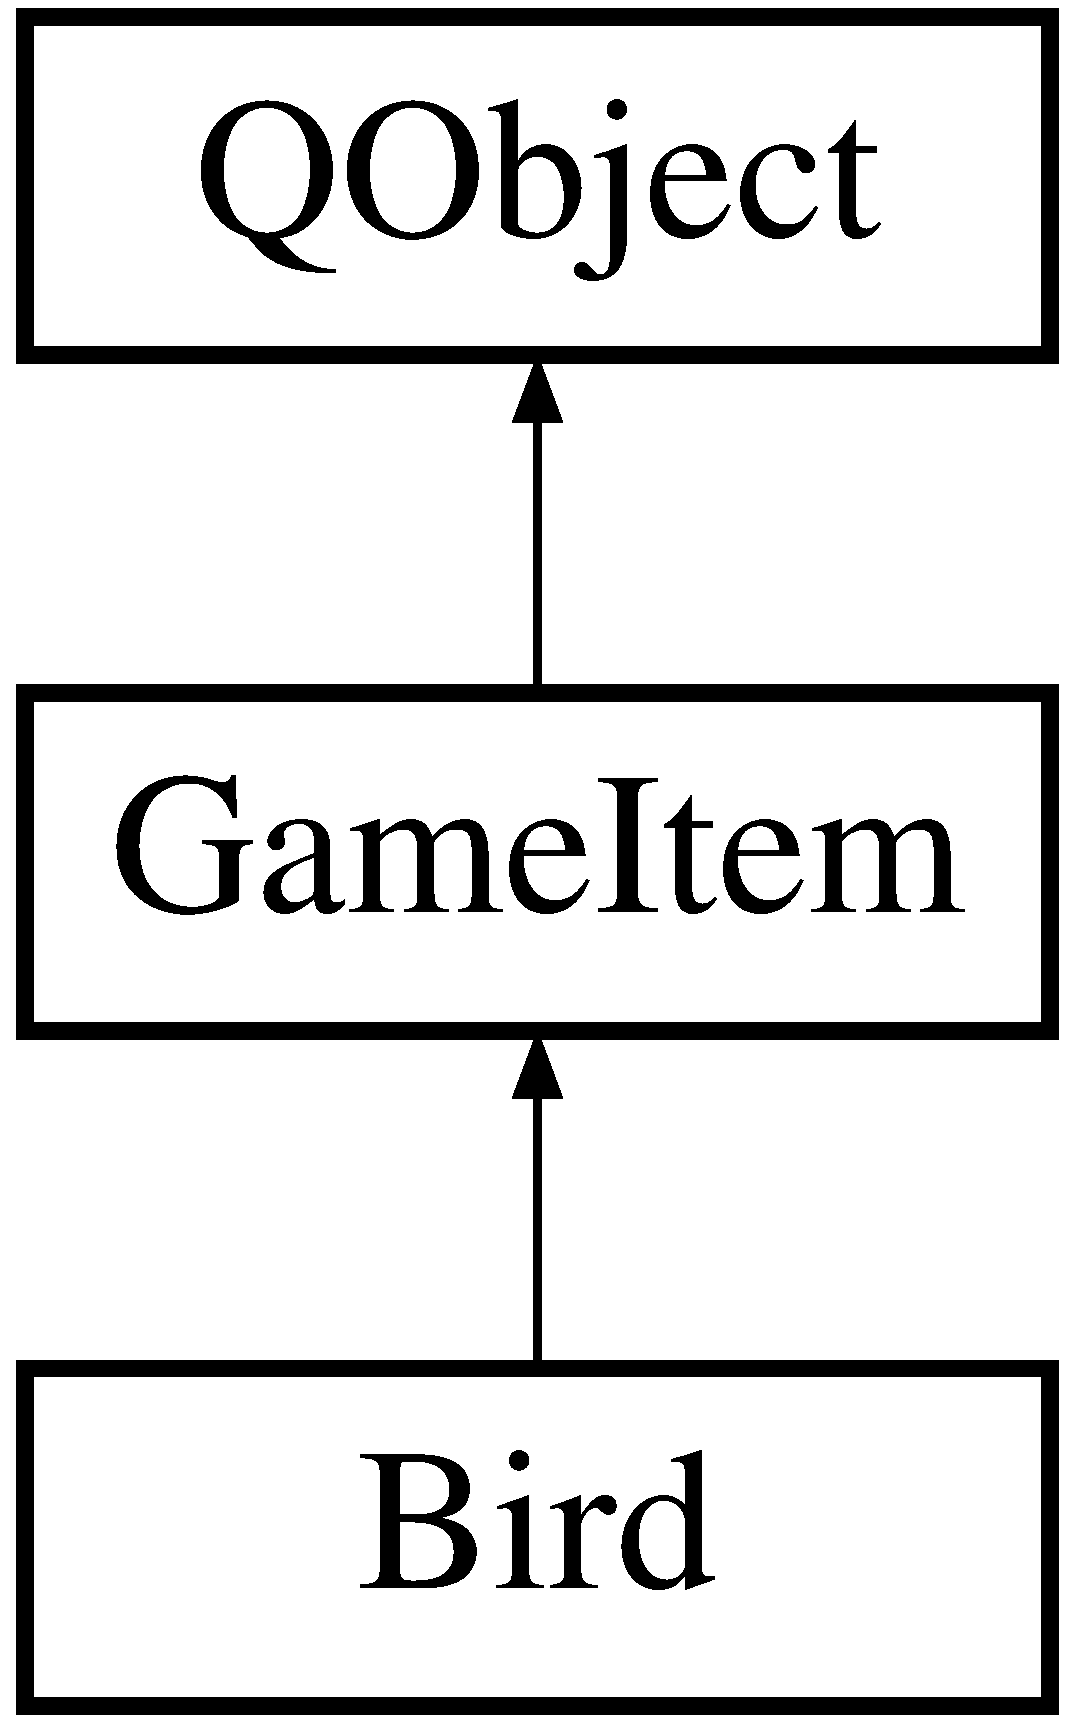
\includegraphics[height=3.000000cm]{classBird}
\end{center}
\end{figure}
\subsection*{Public Slots}
\begin{DoxyCompactItemize}
\item 
\hypertarget{classBird_a2840e2e74ef059b11043ce7306ed7a25}{void {\bfseries paint} ()}\label{classBird_a2840e2e74ef059b11043ce7306ed7a25}

\end{DoxyCompactItemize}
\subsection*{Public Member Functions}
\begin{DoxyCompactItemize}
\item 
\hypertarget{classBird_ac323f5c2088454395569e8580d7c9a41}{{\bfseries Bird} (float x, float y, float radius, Q\-Timer $\ast$timer, Q\-Pixmap pixmap, b2\-World $\ast$world, Q\-Graphics\-Scene $\ast$scene, bool dtype=true)}\label{classBird_ac323f5c2088454395569e8580d7c9a41}

\item 
\hypertarget{classBird_a30a2480db9cbbbc498ab3ce651e579d8}{void {\bfseries set\-Linear\-Velocity} (b2\-Vec2 velocity)}\label{classBird_a30a2480db9cbbbc498ab3ce651e579d8}

\item 
\hypertarget{classBird_ac24711e054b0af39d40aa4ecd8b7e477}{b2\-Vec2 {\bfseries get\-\_\-\-Position} ()}\label{classBird_ac24711e054b0af39d40aa4ecd8b7e477}

\end{DoxyCompactItemize}
\subsection*{Additional Inherited Members}


The documentation for this class was generated from the following files\-:\begin{DoxyCompactItemize}
\item 
bird.\-h\item 
bird.\-cpp\end{DoxyCompactItemize}

\hypertarget{classGameItem}{\section{Game\-Item Class Reference}
\label{classGameItem}\index{Game\-Item@{Game\-Item}}
}
Inheritance diagram for Game\-Item\-:\begin{figure}[H]
\begin{center}
\leavevmode
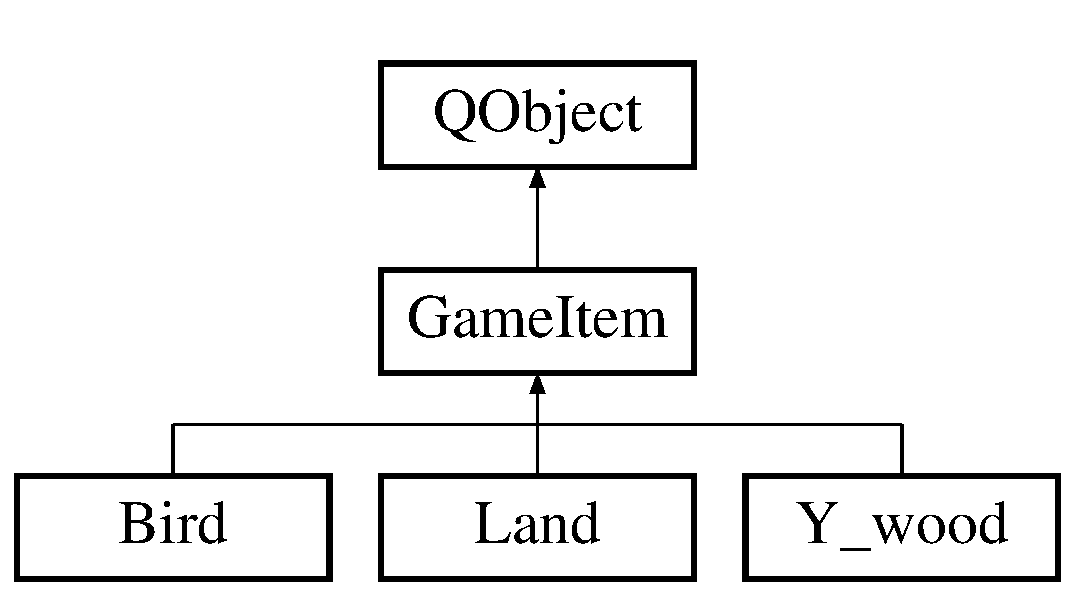
\includegraphics[height=3.000000cm]{classGameItem}
\end{center}
\end{figure}
\subsection*{Public Slots}
\begin{DoxyCompactItemize}
\item 
\hypertarget{classGameItem_a579065cc7a90d31ad5d17b8b6feddabb}{void {\bfseries paint} ()}\label{classGameItem_a579065cc7a90d31ad5d17b8b6feddabb}

\end{DoxyCompactItemize}
\subsection*{Public Member Functions}
\begin{DoxyCompactItemize}
\item 
\hypertarget{classGameItem_a6d2b35fc97b11e0c9fd0105320cea69f}{{\bfseries Game\-Item} (b2\-World $\ast$world)}\label{classGameItem_a6d2b35fc97b11e0c9fd0105320cea69f}

\end{DoxyCompactItemize}
\subsection*{Static Public Member Functions}
\begin{DoxyCompactItemize}
\item 
\hypertarget{classGameItem_aa82bd0ad63ecb3ca6587707c3998d2e8}{static void {\bfseries set\-Global\-Size} (Q\-Size\-F worldsize, Q\-Size\-F windowsize)}\label{classGameItem_aa82bd0ad63ecb3ca6587707c3998d2e8}

\end{DoxyCompactItemize}
\subsection*{Public Attributes}
\begin{DoxyCompactItemize}
\item 
\hypertarget{classGameItem_a3ee0fcf85f92718f1baaa3b76419c2fb}{Q\-Point\-F {\bfseries n\-\_\-mapped\-Point}}\label{classGameItem_a3ee0fcf85f92718f1baaa3b76419c2fb}

\item 
\hypertarget{classGameItem_aa021d911802e721b49270fe790d5e605}{b2\-Body $\ast$ {\bfseries g\-\_\-body}}\label{classGameItem_aa021d911802e721b49270fe790d5e605}

\end{DoxyCompactItemize}
\subsection*{Protected Attributes}
\begin{DoxyCompactItemize}
\item 
\hypertarget{classGameItem_ae01ffe4691dbeef8e2b89949061688ae}{Q\-Graphics\-Pixmap\-Item {\bfseries g\-\_\-pixmap}}\label{classGameItem_ae01ffe4691dbeef8e2b89949061688ae}

\item 
\hypertarget{classGameItem_a7d359356b75422daf7589718358a53f0}{Q\-Size\-F {\bfseries g\-\_\-size}}\label{classGameItem_a7d359356b75422daf7589718358a53f0}

\item 
\hypertarget{classGameItem_a4eea6373f6df167a191100826fa0c151}{b2\-World $\ast$ {\bfseries g\-\_\-world}}\label{classGameItem_a4eea6373f6df167a191100826fa0c151}

\item 
\hypertarget{classGameItem_a3794162e832b8b7779a3dd5a61e62d9d}{bool {\bfseries dragable}}\label{classGameItem_a3794162e832b8b7779a3dd5a61e62d9d}

\end{DoxyCompactItemize}
\subsection*{Static Protected Attributes}
\begin{DoxyCompactItemize}
\item 
\hypertarget{classGameItem_afc553cb4c7c10569dd0fc54e49173e95}{static Q\-Size\-F {\bfseries g\-\_\-worldsize} = Q\-Size\-F()}\label{classGameItem_afc553cb4c7c10569dd0fc54e49173e95}

\item 
\hypertarget{classGameItem_a32623c6e1c31a1a3976bb717c1782a86}{static Q\-Size\-F {\bfseries g\-\_\-windowsize} = Q\-Size\-F()}\label{classGameItem_a32623c6e1c31a1a3976bb717c1782a86}

\end{DoxyCompactItemize}


The documentation for this class was generated from the following files\-:\begin{DoxyCompactItemize}
\item 
gameitem.\-h\item 
gameitem.\-cpp\end{DoxyCompactItemize}

\hypertarget{classLand}{\section{Land Class Reference}
\label{classLand}\index{Land@{Land}}
}
Inheritance diagram for Land\-:\begin{figure}[H]
\begin{center}
\leavevmode
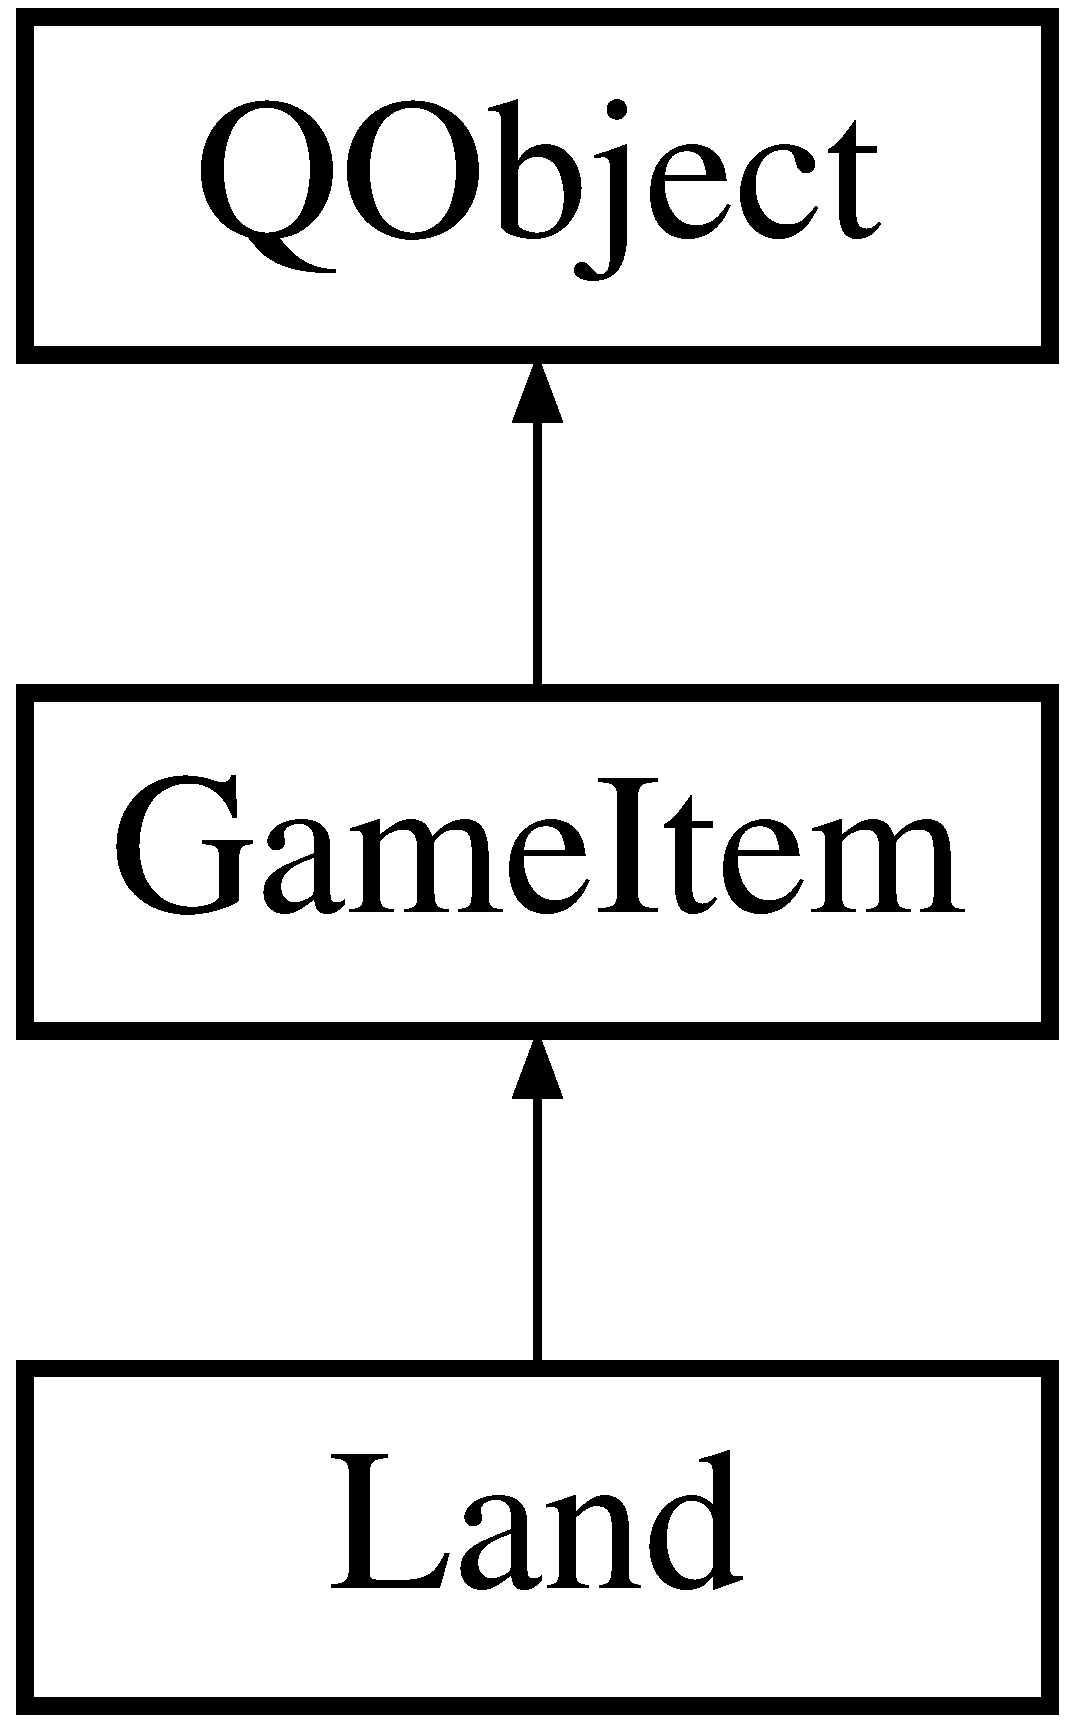
\includegraphics[height=3.000000cm]{classLand}
\end{center}
\end{figure}
\subsection*{Public Member Functions}
\begin{DoxyCompactItemize}
\item 
\hypertarget{classLand_af64ca60994a44576509387d0bf5cb299}{{\bfseries Land} (float x, float y, float w, float h, Q\-Pixmap pixmap, b2\-World $\ast$world, Q\-Graphics\-Scene $\ast$scene)}\label{classLand_af64ca60994a44576509387d0bf5cb299}

\end{DoxyCompactItemize}
\subsection*{Additional Inherited Members}


The documentation for this class was generated from the following files\-:\begin{DoxyCompactItemize}
\item 
land.\-h\item 
land.\-cpp\end{DoxyCompactItemize}

\hypertarget{structqt__meta__stringdata__GameItem__t}{\section{qt\-\_\-meta\-\_\-stringdata\-\_\-\-Game\-Item\-\_\-t Struct Reference}
\label{structqt__meta__stringdata__GameItem__t}\index{qt\-\_\-meta\-\_\-stringdata\-\_\-\-Game\-Item\-\_\-t@{qt\-\_\-meta\-\_\-stringdata\-\_\-\-Game\-Item\-\_\-t}}
}
\subsection*{Public Attributes}
\begin{DoxyCompactItemize}
\item 
\hypertarget{structqt__meta__stringdata__GameItem__t_a6d899d168e51660ea57dd55d93245086}{Q\-Byte\-Array\-Data {\bfseries data} \mbox{[}3\mbox{]}}\label{structqt__meta__stringdata__GameItem__t_a6d899d168e51660ea57dd55d93245086}

\item 
\hypertarget{structqt__meta__stringdata__GameItem__t_a80061230554b89670ec7e225fd325b55}{char {\bfseries stringdata0} \mbox{[}16\mbox{]}}\label{structqt__meta__stringdata__GameItem__t_a80061230554b89670ec7e225fd325b55}

\end{DoxyCompactItemize}


The documentation for this struct was generated from the following file\-:\begin{DoxyCompactItemize}
\item 
moc\-\_\-gameitem.\-cpp\end{DoxyCompactItemize}

\hypertarget{structqt__meta__stringdata__Widget__t}{\section{qt\-\_\-meta\-\_\-stringdata\-\_\-\-Widget\-\_\-t Struct Reference}
\label{structqt__meta__stringdata__Widget__t}\index{qt\-\_\-meta\-\_\-stringdata\-\_\-\-Widget\-\_\-t@{qt\-\_\-meta\-\_\-stringdata\-\_\-\-Widget\-\_\-t}}
}
\subsection*{Public Attributes}
\begin{DoxyCompactItemize}
\item 
\hypertarget{structqt__meta__stringdata__Widget__t_aa12dab415e0beb2f05cbf0528257e748}{Q\-Byte\-Array\-Data {\bfseries data} \mbox{[}8\mbox{]}}\label{structqt__meta__stringdata__Widget__t_aa12dab415e0beb2f05cbf0528257e748}

\item 
\hypertarget{structqt__meta__stringdata__Widget__t_ada88879adfccc3cda0f118440f84f73f}{char {\bfseries stringdata0} \mbox{[}72\mbox{]}}\label{structqt__meta__stringdata__Widget__t_ada88879adfccc3cda0f118440f84f73f}

\end{DoxyCompactItemize}


The documentation for this struct was generated from the following file\-:\begin{DoxyCompactItemize}
\item 
moc\-\_\-widget.\-cpp\end{DoxyCompactItemize}

\hypertarget{classUi__Widget}{\section{Ui\-\_\-\-Widget Class Reference}
\label{classUi__Widget}\index{Ui\-\_\-\-Widget@{Ui\-\_\-\-Widget}}
}
Inheritance diagram for Ui\-\_\-\-Widget\-:\begin{figure}[H]
\begin{center}
\leavevmode
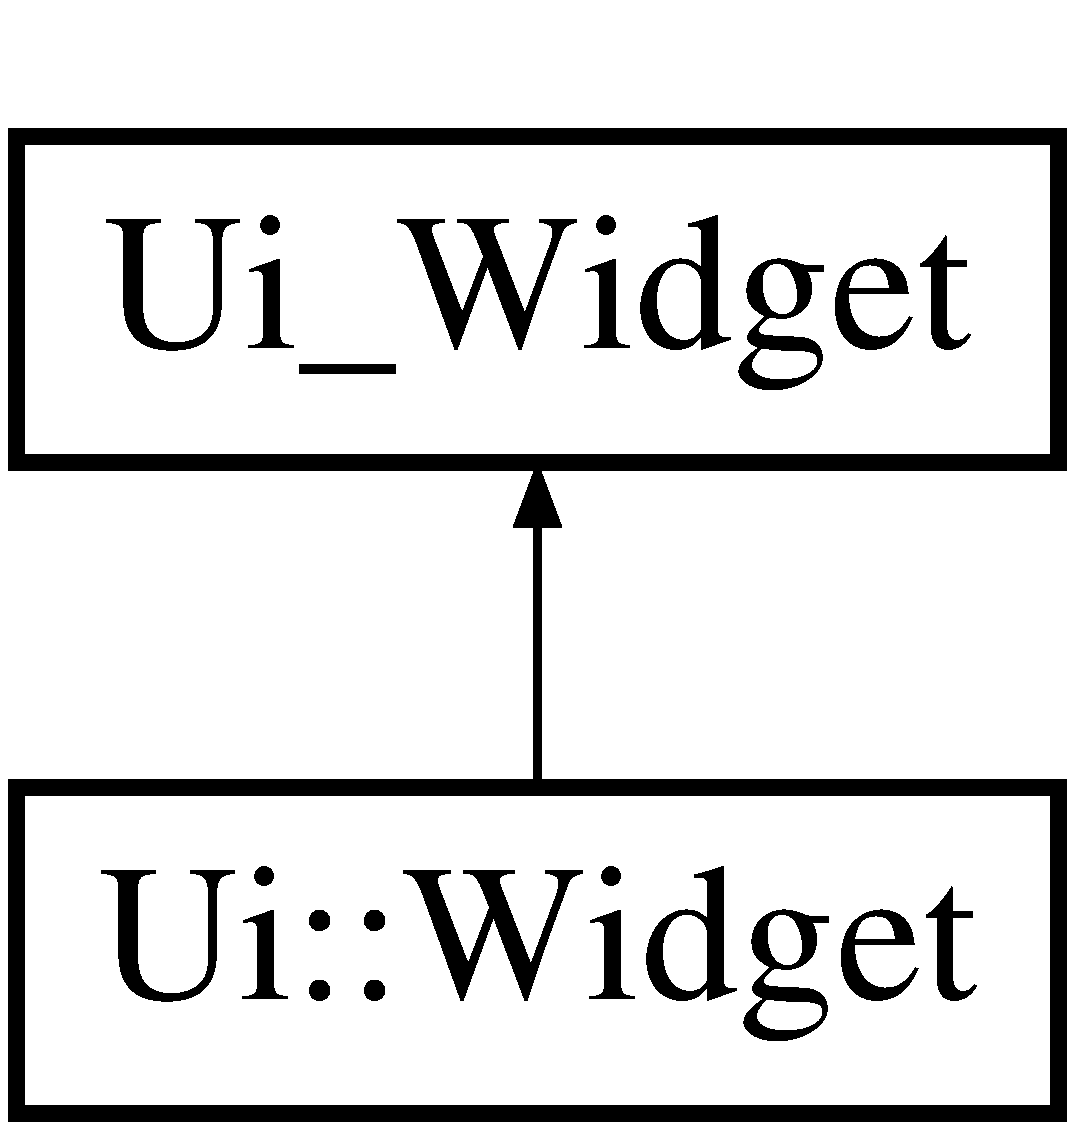
\includegraphics[height=2.000000cm]{classUi__Widget}
\end{center}
\end{figure}
\subsection*{Public Member Functions}
\begin{DoxyCompactItemize}
\item 
\hypertarget{classUi__Widget_a9039ed8704971418cbe19ef8c9eea266}{void {\bfseries setup\-Ui} (Q\-Widget $\ast$\hyperlink{classWidget}{Widget})}\label{classUi__Widget_a9039ed8704971418cbe19ef8c9eea266}

\item 
\hypertarget{classUi__Widget_ae1cb85db8d3658df8dcd104361edcecb}{void {\bfseries retranslate\-Ui} (Q\-Widget $\ast$\hyperlink{classWidget}{Widget})}\label{classUi__Widget_ae1cb85db8d3658df8dcd104361edcecb}

\end{DoxyCompactItemize}
\subsection*{Public Attributes}
\begin{DoxyCompactItemize}
\item 
\hypertarget{classUi__Widget_ab3f8524a48e84bc0ff069bb0b5df5f77}{Q\-Stacked\-Widget $\ast$ {\bfseries stacked\-Widget}}\label{classUi__Widget_ab3f8524a48e84bc0ff069bb0b5df5f77}

\item 
\hypertarget{classUi__Widget_a09f6fcea73c4bc83c6b94547da0bd00e}{Q\-Widget $\ast$ {\bfseries welcome}}\label{classUi__Widget_a09f6fcea73c4bc83c6b94547da0bd00e}

\item 
\hypertarget{classUi__Widget_a934ad5293e23664ac7860b1a526c46bc}{Q\-Label $\ast$ {\bfseries B\-G}}\label{classUi__Widget_a934ad5293e23664ac7860b1a526c46bc}

\item 
\hypertarget{classUi__Widget_a459a60d23ae04ccf2832346cdb7bbfa6}{Q\-Push\-Button $\ast$ {\bfseries S\-T\-A\-R\-T}}\label{classUi__Widget_a459a60d23ae04ccf2832346cdb7bbfa6}

\item 
\hypertarget{classUi__Widget_a1d0ac3f33786d9a4a641c5a4c5f32918}{Q\-Push\-Button $\ast$ {\bfseries E\-X\-I\-T}}\label{classUi__Widget_a1d0ac3f33786d9a4a641c5a4c5f32918}

\item 
\hypertarget{classUi__Widget_a474f01392a601d6e803d20883051b778}{Q\-Widget $\ast$ {\bfseries game}}\label{classUi__Widget_a474f01392a601d6e803d20883051b778}

\item 
\hypertarget{classUi__Widget_a16341716ac1ccd38cb37d395ccf4e709}{Q\-Graphics\-View $\ast$ {\bfseries graphics\-View}}\label{classUi__Widget_a16341716ac1ccd38cb37d395ccf4e709}

\item 
\hypertarget{classUi__Widget_a7dcf5da8902069415662905e93b0d5cb}{Q\-Push\-Button $\ast$ {\bfseries push\-Button}}\label{classUi__Widget_a7dcf5da8902069415662905e93b0d5cb}

\end{DoxyCompactItemize}


The documentation for this class was generated from the following file\-:\begin{DoxyCompactItemize}
\item 
ui\-\_\-widget.\-h\end{DoxyCompactItemize}

\hypertarget{classWidget}{\section{Widget Class Reference}
\label{classWidget}\index{Widget@{Widget}}
}
Inheritance diagram for Widget\-:\begin{figure}[H]
\begin{center}
\leavevmode
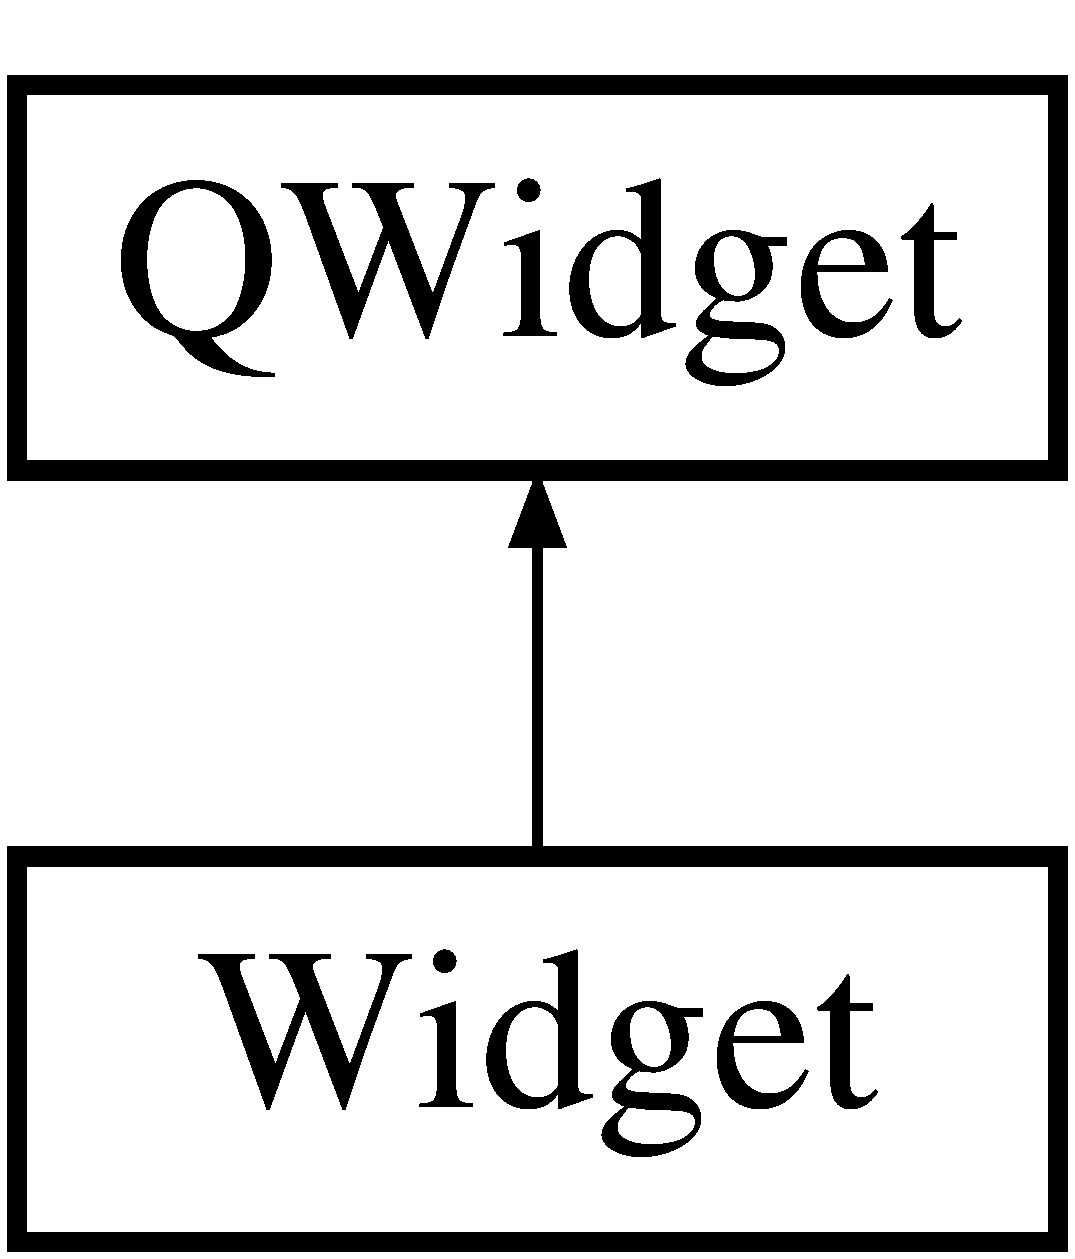
\includegraphics[height=2.000000cm]{classWidget}
\end{center}
\end{figure}
\subsection*{Signals}
\begin{DoxyCompactItemize}
\item 
\hypertarget{classWidget_a2b618e77aff63e7bc4dca1108b1bd889}{void {\bfseries quit\-Game} ()}\label{classWidget_a2b618e77aff63e7bc4dca1108b1bd889}

\end{DoxyCompactItemize}
\subsection*{Public Member Functions}
\begin{DoxyCompactItemize}
\item 
\hypertarget{classWidget_a29531c7f141e461322981b3b579d4590}{{\bfseries Widget} (Q\-Widget $\ast$parent=0)}\label{classWidget_a29531c7f141e461322981b3b579d4590}

\item 
\hypertarget{classWidget_a04fdadbe60fb6ae123c11c3385cb7015}{void {\bfseries close\-Event} (Q\-Close\-Event $\ast$)}\label{classWidget_a04fdadbe60fb6ae123c11c3385cb7015}

\item 
\hypertarget{classWidget_a6da43b19f7b57a59d2a08c6488217c98}{void {\bfseries shoot\-Bird} (float x, float y, float vx, float vy, int bird\-Type)}\label{classWidget_a6da43b19f7b57a59d2a08c6488217c98}

\item 
\hypertarget{classWidget_ab85855521cc554efe43241d061ce7dbd}{bool {\bfseries event\-Filter} (Q\-Object $\ast$, Q\-Event $\ast$event)}\label{classWidget_ab85855521cc554efe43241d061ce7dbd}

\end{DoxyCompactItemize}
\subsection*{Protected Member Functions}
\begin{DoxyCompactItemize}
\item 
\hypertarget{classWidget_a96b48889b8c1b29ecb2804008fbc89be}{void {\bfseries key\-Press\-Event} (Q\-Key\-Event $\ast$e)}\label{classWidget_a96b48889b8c1b29ecb2804008fbc89be}

\end{DoxyCompactItemize}


The documentation for this class was generated from the following files\-:\begin{DoxyCompactItemize}
\item 
widget.\-h\item 
moc\-\_\-widget.\-cpp\item 
widget.\-cpp\end{DoxyCompactItemize}

\hypertarget{classUi_1_1Widget}{\section{Ui\-:\-:Widget Class Reference}
\label{classUi_1_1Widget}\index{Ui\-::\-Widget@{Ui\-::\-Widget}}
}
Inheritance diagram for Ui\-:\-:Widget\-:\begin{figure}[H]
\begin{center}
\leavevmode
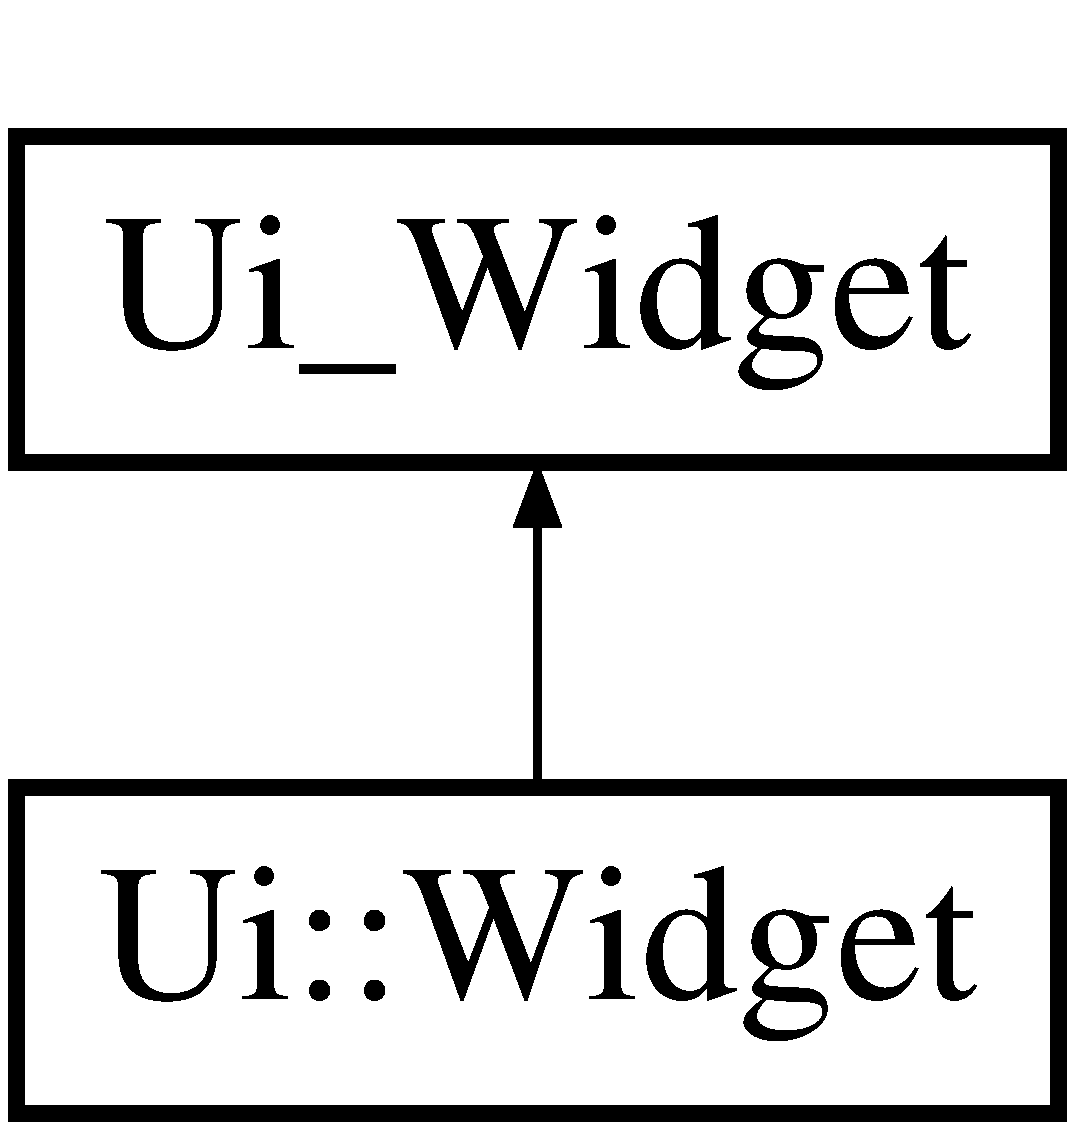
\includegraphics[height=2.000000cm]{classUi_1_1Widget}
\end{center}
\end{figure}
\subsection*{Additional Inherited Members}


The documentation for this class was generated from the following file\-:\begin{DoxyCompactItemize}
\item 
ui\-\_\-widget.\-h\end{DoxyCompactItemize}

\hypertarget{classY__wood}{\section{Y\-\_\-wood Class Reference}
\label{classY__wood}\index{Y\-\_\-wood@{Y\-\_\-wood}}
}
Inheritance diagram for Y\-\_\-wood\-:\begin{figure}[H]
\begin{center}
\leavevmode
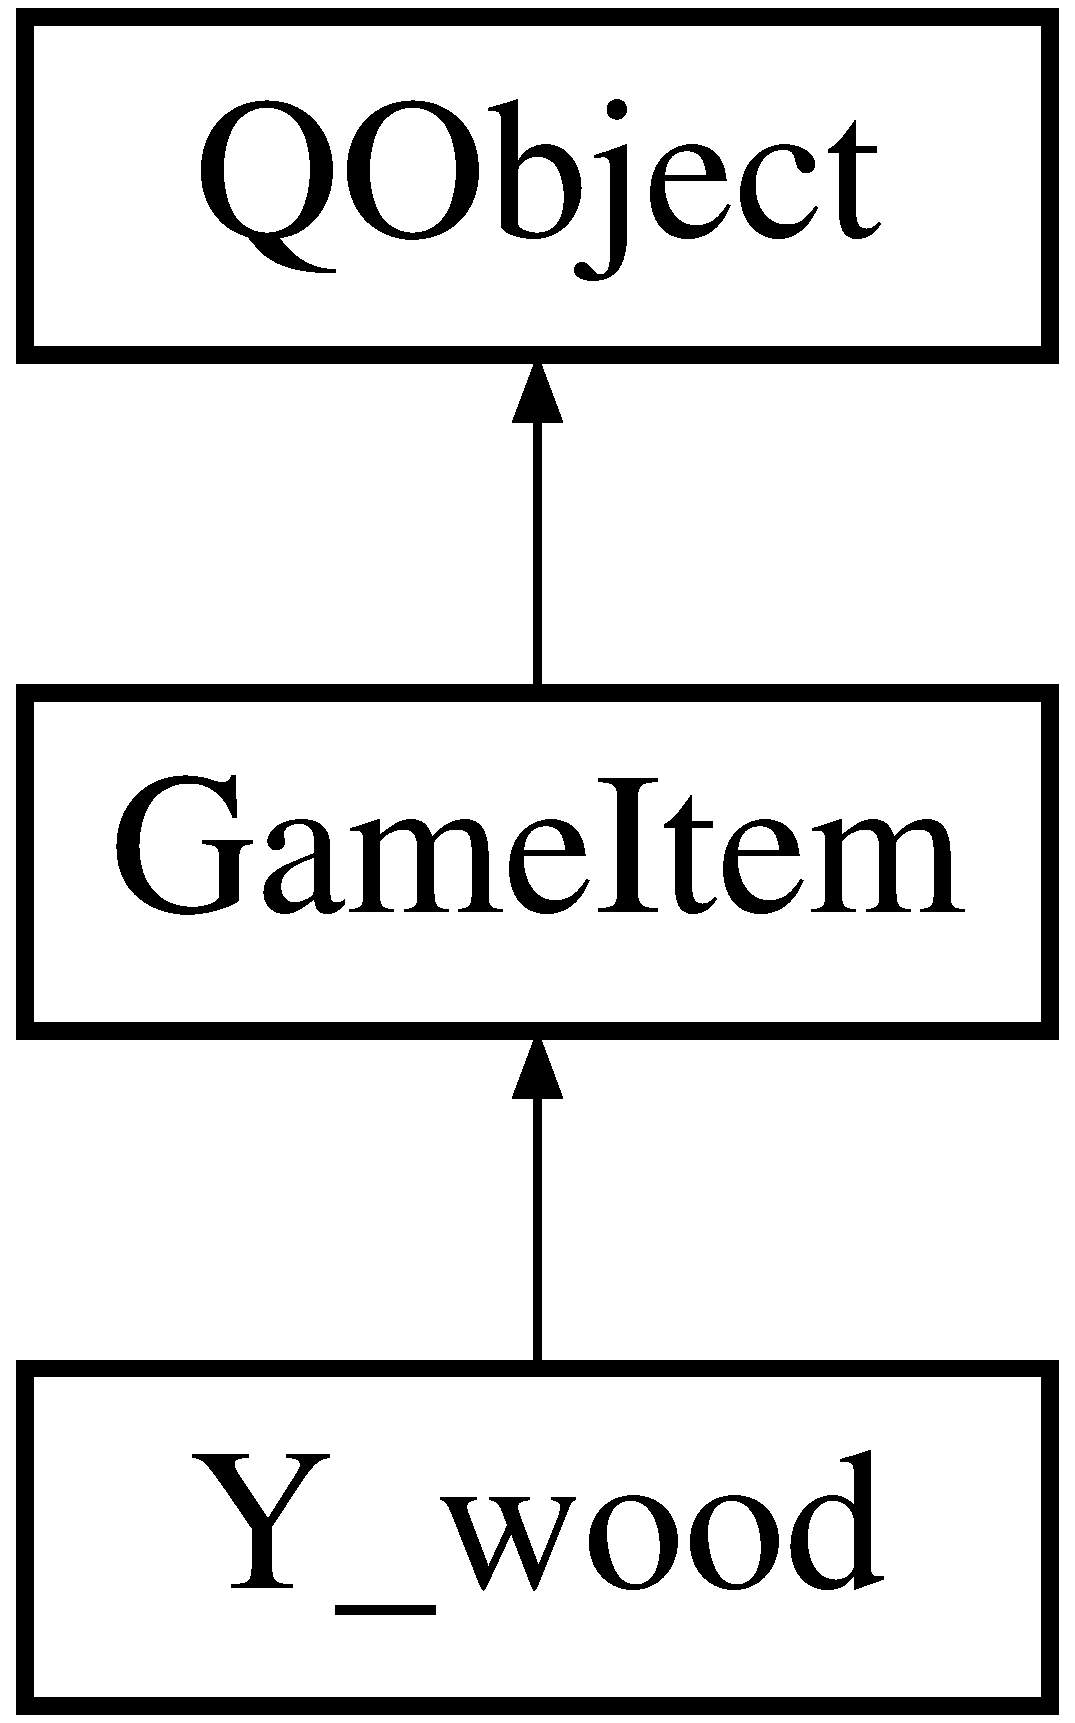
\includegraphics[height=3.000000cm]{classY__wood}
\end{center}
\end{figure}
\subsection*{Public Member Functions}
\begin{DoxyCompactItemize}
\item 
\hypertarget{classY__wood_ad9a8c0af8aa4d0b4243ac41d3404065a}{{\bfseries Y\-\_\-wood} (float x, float y, float w, float h, Q\-Pixmap pixmap, b2\-World $\ast$world, Q\-Graphics\-Scene $\ast$scene)}\label{classY__wood_ad9a8c0af8aa4d0b4243ac41d3404065a}

\end{DoxyCompactItemize}
\subsection*{Additional Inherited Members}


The documentation for this class was generated from the following files\-:\begin{DoxyCompactItemize}
\item 
y\-\_\-wood.\-h\item 
y\-\_\-wood.\-cpp\end{DoxyCompactItemize}

%--- End generated contents ---

% Index
\newpage
\phantomsection
\addcontentsline{toc}{part}{Index}
\printindex

\end{document}
